\documentclass{standalone}
\usepackage{graphicx}	
\usepackage{amssymb, amsmath}
\usepackage{color}

\usepackage{tikz}
\usetikzlibrary{intersections, backgrounds, math}
\usepackage{pgfmath}

\definecolor{light}{RGB}{220, 188, 188}
\definecolor{mid}{RGB}{185, 124, 124}
\definecolor{dark}{RGB}{143, 39, 39}
\definecolor{highlight}{RGB}{180, 31, 180}
\definecolor{light_teal}{RGB}{107, 142, 142}
\definecolor{mid_teal}{RGB}{72, 117, 117}
\definecolor{dark_teal}{RGB}{29, 79, 79}
\definecolor{gray10}{gray}{0.1}
\definecolor{gray20}{gray}{0.2}
\definecolor{gray30}{gray}{0.3}
\definecolor{gray40}{gray}{0.4}
\definecolor{gray60}{gray}{0.6}
\definecolor{gray70}{gray}{0.7}
\definecolor{gray80}{gray}{0.8}
\definecolor{gray90}{gray}{0.9}
\definecolor{gray95}{gray}{0.95}

\begin{document}

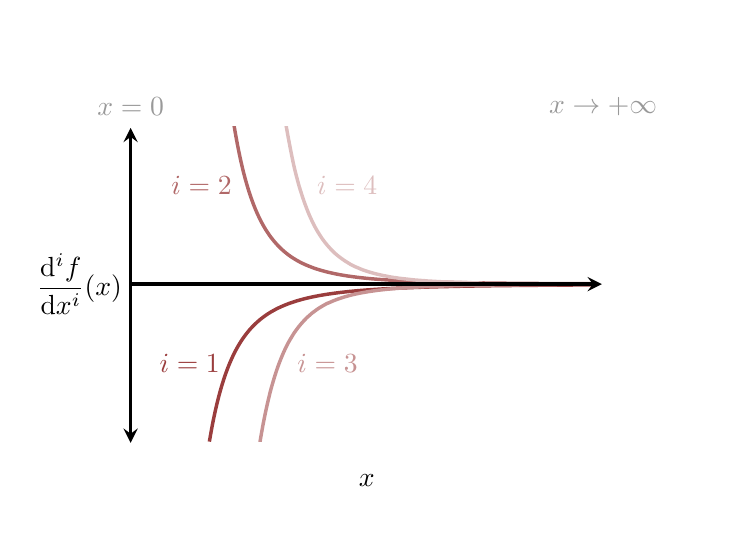
\begin{tikzpicture}[scale=1.0]

   \pgfmathsetmacro{\ys}{0.31};

  \begin{scope}[shift={(8.5, 0)}]
    \draw[white] (-4.25, -3) rectangle (4.25, 3.25);
    
    \begin{scope}
      \clip (-3, -2) rectangle (3, 2);
      
      %
      \pgfmathsetmacro{\prop}{90};
      \colorlet{custom}{dark!\prop!white};
          
      \draw[domain={-2:2.85}, smooth, samples=150, line width=1.25, variable=\x, color=custom] 
        plot ({\x}, {-2 * exp(-3 * ln(\x + 3))});
      \node[custom] at (-2.25, -1) { $i = 1$ };
      
      %  
      \pgfmathsetmacro{\prop}{70};
      \colorlet{custom}{dark!\prop!white};
          
      \draw[domain={-2:2.85}, smooth, samples=150, line width=1.25, variable=\x, color=custom] 
        plot ({\x}, {3 * 2 * exp(-4 * ln(\x + 3))});
      \node[custom] at (-2.1, 1.25) { $i = 2$ };
      
      %  
      \pgfmathsetmacro{\prop}{50};
      \colorlet{custom}{dark!\prop!white};
          
      \draw[domain={-2:2.85}, smooth, samples=150, line width=1.25, variable=\x, color=custom] 
        plot ({\x}, {-4 * 3 * 2 * exp(-5 * ln(\x + 3))});
      \node[custom] at (-0.5, -1) { $i = 3$ };
      
      \pgfmathsetmacro{\prop}{30};
      \colorlet{custom}{dark!\prop!white};
          
      \draw[domain={-2:2.85}, smooth, samples=150, line width=1.25, variable=\x, color=custom] 
        plot ({\x}, {5 * 4 * 3 * 2 * exp(-6 * ln(\x + 3))});
      \node[custom] at (-0.25, 1.25) { $i = 4$ };
    
    \end{scope}
    
    \draw [<->, >=stealth, line width=1.25] (-3.00, -2.015) -- +(0, 4);
    \draw [->, >=stealth, line width=1.25] (-3.015, 0) -- +(6, 0);
    
    \node at (-3.65, 0) { $\displaystyle \frac{\mathrm{d}^{i}f}{\mathrm{d}x^{i}}(x)$};
    \node at (0, -2.5) { $x$ };
    \node[gray60] at (-3, 2.25) { $x = 0$ };
    \node[gray60] at (+3, 2.25) { $x \rightarrow +\infty$ };
  \end{scope}

  
\end{tikzpicture}

\end{document}  